\section{Triangulating Noncovex Polyhedra}
\label{sec:triangulating}

\todo{make sure $2\pi$ factor accounted for.}

A triangulation of a three-manifold is a decomposition
of the manifold into tetrahedra.
Often, we wish to represent the three-manifold
with as few tetrahedra as possible \cite{simplify-mesh-1999}.

Discrete three-manifolds are called a \EMPH{polyhedra}. 
A polyhedron is \EMPH{simple} if it does not intersect itself and is homeomorphic to the sphere.
Let $P$ be a a simple polyhedron. An edge $e$ in $P$ is
\EMPH{reflex} the interior angle formed by its two incident faces
is greater than $\pi$.
A vertex is reflex is it is incident to a reflex edge.
See \figref{reflex} for an example.

\begin{figure}[htb]
\centering
\includegraphics[width=.3\textwidth]{meshes/reflex}
\caption{A polyhedron with one reflex edge (blue), the two vertices incident to the blue
edge are reflex vertices.}
\label{fig:reflex}
\end{figure}

Let $n$ be the number of vertices and $r$ the number of reflex edges.
In the worst case, decomposing a polyhedron of genus
zero into convex parts requires $\Omega(n^2)$ convex pieces
\cite{chazelle-lower-1984}.
Chazell and Palios give an
algorithm to triangulate a nonconvex polyhedra with genus
zero \cite{triangulating-polytope-1990}.
 Their algorithm creates a refinement with $O(n+r^2)$ convex parts
in $O(n\log r +r^2\log r)$ time and $O(n+r^2)$ space.
The algorithm first removes $n-4r$ non-reflex or flat vertices
to create a representation of the polyhedra with $O(r)$ vertices.
Then, vertical planes decompose the reduced polyhedra in to
$O(r^2)$ convex cells.

We share an application of the Gauss-Bonnet theorem
given by Chazelle and Shouraboura to show any polyhedron
 of genus $g$ must have at least $g-1$ reflex edges~\cite{tetra-bounds-c-s-1994}.
 This implies that any polyhedron
can be decomposed with $O(n+r^2)$ convex parts, regardless  of 
the genus! Moreover, the bound is tight .


First, we show 

\begin{lemma}\label{lem:reflex-edge}
The number of reflex edges  incident to a vertex $v$  is at least $-k_v.$
\end{lemma}

\begin{proof}

For each vertex, center a sphere at the vertex,
see  \label{fig:sphere-on-vert} for an illustration.
The intersection of the polyhedron and the sphere
gives a `polygon' $P$ with boundary $L$ the sphere consisting of great
circles. 
Scale the sphere to be unit. Then, the length of each arc
in $L$ is equal the the angle incident to $v$, so the total length of $L$ is
the sum of the angles incident to $v$, see \figref{sphere}.

Let $R$ be the number of reflex edges incident to $v$.
If $R$ is zero, then $P$ is convex and has non-negative curvature
so $L\leq 2\pi$. If $R>0,$
reflex edges incident to $v$ correspond to reflex angles in $P$.
If we have a reflex angle in $P$, bisect it and reduce the 
number of reflex angles and obtain a decomposition
of the sphere into at most $R+1$ convex regions,
thus $L\leq 2\pi(R+1)$.

Thus, we have $L=\sum \alpha_f$ and the curvature 
$k_v=2\pi-\sum \alpha_f$ giving
$L=2\pi(1-k_v)$. Combining this with $L\leq 2\pi(R+1)$
gives $-k_v\leq r.$


\end{proof}

\begin{figure}[htb]
        \centering
        \begin{subfigure}[b]{0.35\textwidth}
        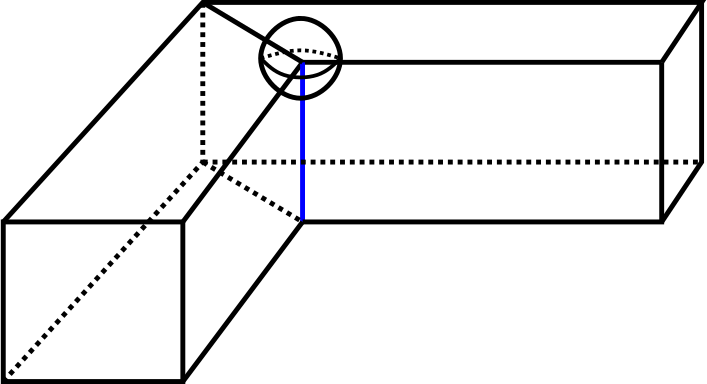
\includegraphics[width=\textwidth]{meshes/reflex-vert-sphere}
        \caption{}
          \label{fig:sphere-on-vert}
        \end{subfigure}
          \hspace{.0cm}
         \begin{subfigure}[b]{0.45\textwidth}
        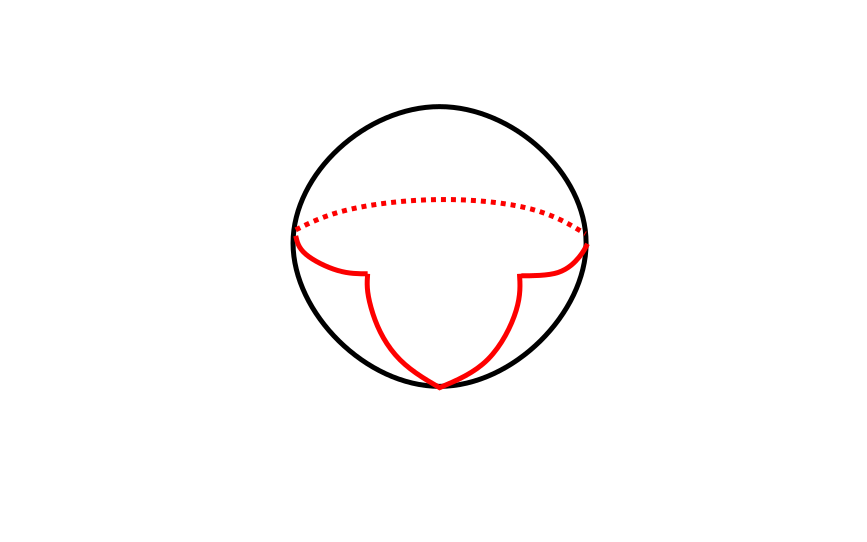
\includegraphics[width=\textwidth]{meshes/sphere-intersection}
        \caption{}
        \label{fig:sphere}
        \end{subfigure}\\
		\caption{(a) A sphere around a reflex vertex. (b) Where the polyhedron
		intersects the sphere.
		\label{fig:sphere}}
\end{figure}


Next, we show
\begin{theorem}[Reflex Angles]\label{thm:reflex}

Any polyhedron of genus $g$ must have 
at least $g-1$ reflex dihedral angles. 

\end{theorem}
\begin{proof}
Let $r$ be the total number of reflex edges in a polyhedra.
By the classification of oriented surfaces, the Euler characteristic 
 is determined by the genus, $\chi=2-2g$.
By \lemref{reflex-edge}, $\sum_v -k_v\leq 2 r$ since each
reflex edge is incident to two vertices.
By the Gauss-Bonnet theorem $\sum_vk_v= 2-2g,$
so $-2r\leq 2-2g$ and $g\leq r+1$ as desired.

\end{proof}

Given a polyhedron of genus $g$, we can temporally 
insert a disk in each essential cycle, creating a polyhedron
of genus zero, we can apply the algorithm to
decompose genus zero polyhedra given in \cite{triangulating-polytope-1990}.
Since we added $g$ disks the algorithm decomposes
the polyhedron into $O(n+ (r+g)^2)$ tetrahedra.
By \thmref{reflex}, $g\leq r+1$ showing that the bound
is still $O(n+r^2)$ regardless of the genus.

